\chapter{Tools from Differential Geometry}\label{ch:tools}

\begin{flushright}
	\emph{People know or dimly perceive, that if thinking is not kept pure and keen, if spirit's contemplation do not holds, even mechanics of automobiles and ships will soon cease to run. Even engineer's slide rule, computations of banks and stock exchanges will wonder aimlessly for the lost of authority, and chaos will ensue.} \\ -Hermann Hesse, \emph{Magister Ludi}
\end{flushright}

% % % % % % % % % % % % % % % % % % % % % % % % % % % % % % % % % % % % % %
% % % % % % % % % % % % % % % % % % % % % % % % % % % % % % % % % % % % % %
% % SECTION
% % % % % % % % % % % % % % % % % % % % % % % % % % % % % % % % % % % % % %
% % % % % % % % % % % % % % % % % % % % % % % % % % % % % % % % % % % % % %
\section{A Lie Group Structure for the Set of Transformation}\label{se:finite_lie_group}

%%introductory definition
We consider every group $\mathbb{G}$ as a group of transformations acting on $\mathbb{R}^{d}$, having in mind the particular case $d=2,3$ for 2-dimensional or 3-dimensional images.
We will focus out attention to transformations defined by matrices or diffeomorphism. Other than group they also have the structure of Lie group: they are considered with a maximal atlas that makes them differentiable manifold, in which the composition of two transformation and the inverse of each transformation are well defined differentiable maps:
\begin{align*}
\mathbb{G} \times \mathbb{G} & \longrightarrow  \mathbb{G}    \\
(x,y) &\longmapsto  x y^{-1}
\end{align*}
Differential geometry is in general a technique to use the well known calculus features and operators on spaces different from the usual $\mathbb{R}^{n}$. Adding the differentiable structure to a group of transformations gives us new handles to hold and manipulate them: in particular provides the opportunity to define a tangent space to each point of the group (and so a fiber bundle), a space of vector fields, a set of flows and one parameter subgroup as well as other features that enrich this structure. The abstract idea of vector field over a manifold will be concretized for image registration introducing the concepts of \emph{displacement field}, \emph{deformation field} and \emph{velocity field (stationary or time varying)} that will be there presented. 
Due to space limitations we will refer to \cite{do1976differential}, \cite{lee2012introduction} for the definitions and concepts of differential geometry and \cite{do1992riemannian} for definition and concepts of Riemannian geometry.\\
Some notes about these topics, tailored for image registration can be found on the github repository \cite{notes_geometry_and_imaging}

% % % % % % % % % % % % % % % % % % % % % % % % % % % % % % % % % % % % % %
% % SECTION
% % % % % % % % % % % % % % % % % % % % % % % % % % % % % % % % % % % % % % 
\section{Lie Exponential, Lie logarithm, Lie log-composition and the BCH formula }\label{se:lie_exp_log_comp_bch}
Let $\mathbf{v}$ be an element in the tangent space $\mathfrak{g}$ and $V\in\mathcal{V}(\mathbb{G})$ the unique vector field defined by $\mathbf{v}$ over a local coordinate system around the origin. Let $\Phi_{V}$ be the flow associated with the vector field and $\gamma(t)$ the unique integral curve of $V$ passing through the identity of the group.  
The \emph{Lie exponential} is defined as (\cite{do1992riemannian}, \cite{ebin2006singularities})
\begin{align*}
\exp :  \mathfrak{g} & \longrightarrow  \mathbb{G}  \\
\mathbf{v} &\longmapsto  \exp(\mathbf{v} ) = \gamma(1) \quad \dot{\gamma}(t) = V_{\gamma(t)}, \gamma(0) = e
\end{align*}
It satisfies the following properties:
\begin{enumerate}
	\item $\exp(\mathbf{v}) = \Phi_{V}(e,1)$.
	\item $\exp(t\mathbf{v}) =\gamma(t) = \Phi_{V}(e,t)$.
	\item $\exp(\mathbf{v}) = e$ if $\mathbf{v} = \mathbf{0}$.
	\item $\exp(\mathbf{v})\circ \exp(\mathbf{-v})  = e$
	\item The exponential function satisfies the one parameter subgroup property:
	\begin{align*}
	\exp((t+s)\mathbf{v}) = \gamma(t+s) = \gamma(t)\circ \gamma(s) = \exp(t\mathbf{v})\exp(s\mathbf{v})
	\end{align*}
	\item $\exp(\mathbf{v})$ is invertible and $(\exp(\mathbf{v}))^{-1} = \exp(-\mathbf{v})$.
	\item $\exp$ is a diffeomorphism between a neighborhood of $\mathbf{0}$ in $\mathfrak{g}$ to a neighborhood of $\text{Id}$ in $\mathbb{G}$.
\end{enumerate}
The neighborhoods of $\mathbb{G}$ and of $\mathfrak{g}$ such that the last property holds, are called \emph{internal cut locus} of $\mathbb{G}$ and $\mathfrak{g}$ respectively. The \emph{cut locus} is the boundary of the internal cut locus\footnote{Here we define cut locus starting from the exp and log function, and in both domains. Traditionally it is defined only on Riemannian manifolds and using the geodesics (see \cite{do1992riemannian}, p. 267). For Levi Civita connection we have that the definition are coincident.}.\\
When we deal with a matrix Lie group of dimension $n$, we have the following remarkable properties:
\begin{enumerate}
	\item for all $\mathbf{v}$ in a matrix Lie algebra $\mathfrak{g}$:
	\begin{align*}
	\exp(\mathbf{v}) = \sum_{k=0}^{\infty} \frac{\mathbf{v}^{k}}{k!}
	\end{align*}
	\item If $\mathbf{u}$ and $\mathbf{v}$ are commutative then $\exp(\mathbf{u} + \mathbf{v}) = \exp(\mathbf{u})\exp(\mathbf{v})$.
	\item If $\mathbf{c}$ is an invertible matrix then $\exp(\mathbf{c}\mathbf{v}\mathbf{c}^{-1}) = \mathbf{c}\exp(\mathbf{v})\mathbf{c}^{-1}$.
	\item $\det(\exp(\mathbf{v})) = \exp(\text{trace}(\mathbf{v}))$
	\item For any norm, $\euclideanMetric{\exp(\mathbf{v})} \leq \exp(\euclideanMetric{\mathbf{v}})$.
	\item  $\exp(\mathbf{u} + \mathbf{v}) =\lim_{m\rightarrow \infty} (\exp(\frac{\mathbf{v}}{m})\exp(\frac{\mathbf{v}}{m}))^{m}$
	\item If $\exp(\mathbf{w}) = \exp(\mathbf{u}) \circ \exp(\mathbf{v})$ then $\exp(\mathbf{-w}) = \exp(\mathbf{-v}) \circ \exp(\mathbf{-u})$.
	\item For $\text{ad}$ adjoint map in the Lie algebra we have $ \exp(\text{Ad}_{\mathbf{u}}\mathbf{v} ) = \text{Ad}_{\mathbf{u}}\exp(\mathbf{v})$
\end{enumerate}
The idea of defining an inverse of the Lie exponential leads to the idea of the Lie logarithm, defined
\begin{align*}
\log : \mathbb{G} & \longrightarrow \mathfrak{g} \\
p &\longmapsto \log (p)  =  \mathbf{v}   
\end{align*}
where $\mathbf{v}  $ is the tangent vector having $p$ as it $\exp$.\\


\noindent
If $\mathbb{G}$ is a matrix Lie group of dimension $n$, the following properties hold:
\begin{enumerate}
	\item for all $\mathbf{v}$ in the matrix Lie algebra $\mathfrak{g}$:
	\begin{align*}
	\log(\mathbf{v}) = \sum_{k=1}^{\infty}(-1)^{k+1} \frac{(\mathbf{v}-I)^{k} }{k!}
	\end{align*}
	where $I$ is the identity matrix.
	\item For any norm, and for any $n\times n$ matrix $\mathbf{c}$, exists an $\alpha$ such that 
	\begin{align*}
	\euclideanMetric{ \log(I + \mathbf{c}) - \mathbf{c} }  \leq \alpha \euclideanMetric{ \mathbf{c}}^{2}
	\end{align*}
	\item For any $n\times n$ matrix $\mathbf{c}$ and for any sequence of matrix $\{\mathbf{d}_{j}\}$ such that  $\euclideanMetric{ \mathbf{d}_{j}} \leq \alpha/j^2$ it follows:
	\begin{align*}
	\lim_{k\rightarrow \infty} \big( I + \frac{\mathbf{c}}{k} + \mathbf{d}_{k} \big)^{k} = \exp{(\mathbf{c})}
	\end{align*}
\end{enumerate} 
Here we may see the beginning of the problem we have to deal with for the rest of the research, when passing from the finite dimensional case to the infinite dimensional case.\\
The domain of the logarithm is the matrix Lie group in which only the composition is defined. Nevertheless it is possible to compute $I + \mathbf{c}$, and this still make sense (and satisfy remarkable properties) when applied to the $\log$. On the other side the domain of the exponential is the matrix Lie algebra, but the exponential can be nevertheless applied to a generic matrix.\\
\emph{This can be done thanks to the fact that for matrices, $\mathfrak{g}$ and $\mathbb{G}$ are subset of a bigger algebra, the algebra of invertible matrix}. In this structure the operation of sum is still defined over the group that admit only compositions. The sum between element of a group can be performed on a Lie group, every time he and its Lie algebra are subset of a bigger algebra \cite{kirillov2008introduction}. In these cases infinite series are doors to pass from the structure of group and the algebra. When presenting the rigid body transformation in chapter \ref{ch:spatial_transformations} we will see another couple of access doors based on numerical approximations.\\

The (extremely) continuous nature of a diffeomorphism is not compatible with the (extremely) discrete nature of computers. It is not possible to implement something that maintains any of the property of diffeomorphism in a computer. As shown in \cite{hernandez2008comparing}, for some parameters the Stationary LDDMM and the diffeomorphic Demons, the transformations involved in diffeomorphic framework may not preserve the signs of the Jacobian determinant. As previously said, the only options we have for practical implementations are the vector fields discretized on a $d$ dimensional grid. In the paper of Arsigny \cite{arsigny2006log}, scaling and squaring and inverse scaling and squaring are proposed for the computation of exponential and logarithm respectively; they transform a vector field in another vector field, and reasonably the domain and codomain of these transformations are radically different from the exp and log function defined for diffeomorphisms. \\
Matrices are much easier to handle, since the Lie group of a Lie algebra is still an algebraic structure defined by matrices, in which products are compatible with the composition. In this case the exponential and logarithm have domain and codomain in the appropriate restriction of the general linear group.\\
Passing from finite dimensional case of matrices to infinite dimensional case of diffeomorphisms requires a way to represent diffeomorphisms having only vector fields to deal with. The strategy here proposed is to embed the Lie group structure $\mathbb{G} = \text{Diff}(\Omega)$ in the Lie algebra $\mathfrak{g} = \mathcal{V}(\Omega)$, whose implementation better reflect the discretization of the diffeomorphisms. This is done toward the definition of an operation, defined on $\mathfrak{g} $, that utilizes the group structure of $\mathbb{G}$ on its elements.\\


We define now the Lie Log-composition (Lie to distinguish it from the Affine Log-composition of the next section) as inner binary operation on the Lie algebra that reflects the composition on the lie group:
\begin{align*}
\oplus : \mathfrak{g} \times \mathfrak{g} & \longrightarrow \mathfrak{g}    \\
(\mathbf{v}_{1}, \mathbf{v}_{2}) &\longmapsto \mathbf{v}_{1}\oplus \mathbf{v}_{2} =  \log(\exp(\mathbf{v}_1)\circ \exp(\mathbf{v}_2))
\end{align*}

\begin{figure}[!ht]
	\centering
	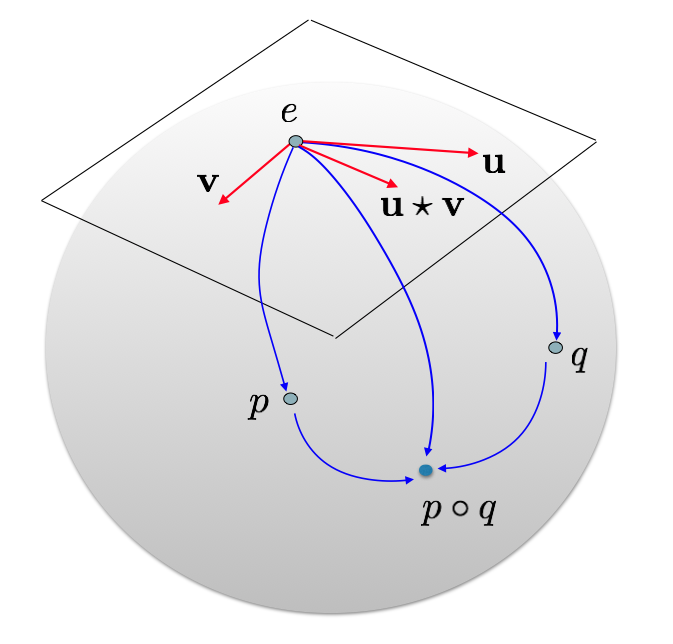
\includegraphics[scale=0.35]{figures/log_composition.png}
	\caption{graphical visualization of the Lie log-composition.}
	\label{fig:composition}
\end{figure}

\noindent
Following properties holds for the Lie log-composition:
\begin{enumerate}
	\item $\mathfrak{g} $ with the Lie log-composition $\oplus$ is a local topological non-commutative group (local group for short): if $C_{\mathfrak{g}}$ is the internal cut locus of $\mathfrak{g}$ then:
	\begin{enumerate}
		\item $(\mathbf{u}_{1}\oplus\mathbf{u}_{2}) \oplus \mathbf{u}_{3}
		= \mathbf{u}_{1}\oplus(\mathbf{u}_{2} \oplus \mathbf{u}_{3})$ for all $\mathbf{u}_{1}, \mathbf{u}_{2}, \mathbf{u}_{3}$ in $C_{\mathfrak{g}}$.
		\item $\mathbf{u}\oplus\mathbf{0}  = \mathbf{0}\oplus\mathbf{u} = \mathbf{u}$ for all $\mathbf{u}$ in $C_{\mathfrak{g}}$.
		\item $\mathbf{u}\oplus(-\mathbf{u} ) = \mathbf{0}$ for all $\mathbf{u}$ in $C_{\mathfrak{g}}$.
	\end{enumerate}
	\item For all $t,s$ real, such that $(t+s)\mathbf{u}$ is in $C_{\mathfrak{g}}$,
	\begin{align*}
	(t\mathbf{u})\oplus (s\mathbf{u}) = (t+s)\mathbf{u}
	\end{align*}
	And in particular, if the Lie algebra $\mathfrak{g}$ has dimension $1$ the local group structure is compatible with the additive group of the vector space $\mathfrak{g}$.
\end{enumerate}

\noindent
We refer to $(\mathfrak{g} , \oplus)$ as the Lie Log-group. Additional observation of this algebraic structure in the particular case of diffeomorphisms, are contained in the next chapter.\\
To compute the log-composition there is a formula, the BCH (for Lie group \cite{hall2015lie}, general case \cite{wojtynski1994one}, applied to medical imaging \cite{vercauteren08}), that provides the exact solution to the Log-composition. 
\begin{align*}
BCH(\mathbf{u},\mathbf{v}) 
= 
\mathbf{u} + \mathbf{v} + \frac{1}{2}[\mathbf{u},\mathbf{v}] + \frac{1}{12}([\mathbf{u},[\mathbf{u},\mathbf{v}]]
+ [\mathbf{v},[\mathbf{v},\mathbf{u}]]) - \frac{1}{24}[\mathbf{v},[\mathbf{u},[\mathbf{u},\mathbf{v}]]] +... 
\end{align*}
It consists of an infinite series of Lie bracket whose asymptotic behaviour cannot be predicted only from the coefficient of each nested Lie bracket term. In practical applications it can be computed using its \emph{approximation of degree} $k$, defined as the sum of the BCH terms having no more than $k$ nested Lie bracket. For example:
\begin{align*}
BCH^{0}(\mathbf{u},\mathbf{v}) &= \mathbf{u} + \mathbf{v} \\
BCH^{1}(\mathbf{u},\mathbf{v}) &=  \mathbf{u} + \mathbf{v} + \frac{1}{2}[\mathbf{u},\mathbf{v}] \\
BCH^{2}(\mathbf{u},\mathbf{v}) &=  \mathbf{u} + \mathbf{v} + \frac{1}{2}[\mathbf{u},\mathbf{v}] + \frac{1}{12}([\mathbf{u},[\mathbf{u},\mathbf{v}]] + [\mathbf{v},[\mathbf{v},\mathbf{u}]])
\end{align*}
These numerical approximations of the group composition leave the difficulty of managing the problem of the error carried by each term.


% % % % % % % % % % % % % % % % % % % % % % % % % % % % % % % % % % % % % %
% % SECTION
% % % % % % % % % % % % % % % % % % % % % % % % % % % % % % % % % % % % % % 
\section{Affine Exponential, Affine logarithm and affine log-composition}\label{se:affine_exp_log_comp}

Considering a Lie Group $\mathbb{G}$ with a connection $\nabla$ (that provides geodesics and curvature over manifold on which no Riemannian metric has been defined, see \cite{do1992riemannian}), the vector field $\nabla_{U}(V)$ associates at each point of the manifold the projection on the tangent plane of the covariant derivative of $U$ in the direction of $V$. \\
First consequence of the definition of the connection is the possibility of define \emph{geodesics} between points $p$ and $q$ of the manifold. A geodesic is a curve $\gamma$ such that:
\begin{align*}
\gamma:[0,1] \longrightarrow \mathbb{G} \qquad \gamma(0)=p,~ \gamma(1) = p,~ \nabla_{\dot{\gamma}}\dot{\gamma} = 0 
\end{align*} 
Note that in this case the concept of geodesic did not involves any metric defined on the surface of the manifold. If also a Riemannian metric is defined on $\mathbb{G} $, then geodesics defined by the metric coincides with the geodesics defined by the connection only for the particular Levi-Civita connection (see \cite{do1992riemannian}).
A connection is said to be left invariant if it is closed for left invariant vector fields, i.e. if for any $V, W \in Left\mathcal{V}(\mathbb{G}) $ their connection $ \nabla_{U}V$ is still left invariant.\\

\noindent
Second straight consequence of the definition of connection allows us to define a new kind of exponential from the Lie algebra to the Lie group that relies on the concept of geodesics. This time the tangent plane that defines the Lie algebra is considered at the point $p$ of the Lie group and $\mathbf{v} \in T_{p}\mathbb{G}\simeq \mathfrak{g}$ is a tangent vector at the point $p$: 
\begin{align*}
\exp :  \mathbb{G}  \times \mathfrak{g}     &\longrightarrow \mathbb{G}  
\\ 
(p,\mathbf{v}) &\longmapsto \exp_{p}(\mathbf{v})  = \gamma(1; p,\mathbf{v})
\end{align*}
The curve $\gamma(t;p,\mathbf{v}) = \gamma(t)$ on $\mathbb{G}$ is the unique one with the following features:  
\begin{align*}
\gamma(0) = p\qquad  \dot{\gamma}(0) =  \mathbf{v} \qquad \nabla_{\dot{\gamma}}\dot{\gamma} = 0 
\end{align*}
This second kind of exponential is called affine exponential\footnote{
	Note on the notation: to distinguish the affine $\exp$ and $\log$ from the Lie $\exp$ and $\log$ presented in the previous section, the affine will always have the subscript of the point of application even when it is the identity.
	}
The following properties hold:
\begin{enumerate}
	\item If $\nabla$ is a Cartan connection then $\exp_{e}$ and $\exp$ coincides.
	\item For all $p$ in $\mathbb{G}$, $\mathbf{v} \in T_{p}\mathbb{G}$ and $t$ real
	\begin{align*}
	\exp _{p}(t\mathbf{v})  = \gamma(t; p,\mathbf{v})
	\end{align*}
	\item Given $\mathbf{u} \in T_{e}\mathbb{G}$, $\mathbf{v} \in T_{\exp _{e}(\mathbf{u})}\mathbb{G}$, exists a $\mathbf{w} \in T_{e}\mathbb{G}$ such that 
	\begin{align*}
	\exp_{e}(\mathbf{w})  = \exp_{\exp _{e}(\mathbf{u})}(\mathbf{v}) \circ  \exp _{e}(\mathbf{u})
	\end{align*}
	\item If $V$ is a unitary left-invariant vector field, then for $V_{e} \in T_{e}\mathbb{G}$
	\begin{align*}
	\exp_{e}(2V_{e})  = \exp_{\exp _{e}(V_{e})}(V_{\exp _{e}(V_{e})}) \circ  \exp _{e}(V_{e})
	\end{align*}
\end{enumerate}
Last two properties provides the intuitive idea that it is possible to move on the fiber bundle of the Lie group transporting in some sense a tangent vector defined at the identity on another tangent space. Certainly the Lie group possess a unique Lie algebra, as the tangent space at some point (the group's identity by convention), but two different tangent space (so two times the same Lie algebra structure) may not be oriented in the same way. \\

\noindent
To approach the inverse of the affine exponential we consider the affine logarithm:
\begin{align*}
\log :  \mathbb{G}  \times \mathbb{G}   \longrightarrow T_{p}\mathbb{G}   \simeq \mathfrak{g} 
\\ 
(p,q) \longmapsto \log_{p}(q)  = \mathbf{v} 
\end{align*}
Where $\mathbf{v} $ is the vector at the tangent plane defined at $p$ such that the curve on $\mathbb{G} $ with the following features
\begin{align*}
\gamma(0) = p\qquad  \gamma(1) = q \qquad \nabla_{\dot{\gamma}}\dot{\gamma} = 0 
\end{align*}
has as its tangent in $p$ the vector $\mathbf{v}$.\\

\noindent
Any Lie group $\mathbb{G}$ considered with a left-invariant connection $\nabla$ can be equipped with a metric,  based on the elements of its tangent space and on the log, for example: 
\begin{align*} 
\text{dist}(x,y) := \euclideanMetric{\log_{e}(x^{-1}\circ y) } \qquad \forall x, y \in \mathbb{G}
\end{align*}
This metric is not necessarily coincident with the Riemannian one. \\

Is now time to extend the definition of Log-composition, with the definition of affine logarithm and affine exponential. The first step is to extend the definition of internal cut locus of the Lie algebra, even when not centered at the zero. 
If the tangent space is not considered at $e$ of $\mathbb{G}$ but at some general point $p$, we still have a diffeomorphism between a neighborhood of $\mathbf{0}$ in $\mathfrak{g}$ to a neighborhood of $p$ in $\mathbb{G}$. The internal cut locus of $\mathfrak{g}$ this time is based on $p$ and it is denoted with $C_{\mathfrak{g}}(p)$.\\
\noindent
Given a point $p_1$ and a vector $\mathbf{v}_{1}$ on its tangent space $T_{p_1}\mathbb{G}$, the \emph{affine Log-composition} is defined as the operation $\tilde{\oplus} $ over the fiber bundle of $\mathbb{G}$ such that 
\begin{align*}
\cdot ~ \tilde{\oplus} ~ \mathbf{v}_{1}  : T_{\exp_{p_1}(\mathbf{v}_{1})}\mathbb{G}  & \longrightarrow T_{p_1}\mathbb{G}   
\\
\mathbf{v}_{2}&\longmapsto \mathbf{v}_{2}~\tilde{\oplus}~ \mathbf{v}_{1}
=
\log_{p_1}(\exp_{\exp_{p_1}(\mathbf{v}_{1})}(\mathbf{v}_{2})\circ\exp_{p_1}(\mathbf{v}_{1}))
\end{align*}
Note that not necessarily $\mathbf{v}_{1}~\tilde{\oplus}~ \mathbf{v}_{2}$ is a vector belonging to the internal cut locus based on the starting point $p_{1}$.


% % % % % % % % % % % % % % % % % % % % % % % % % % % % % % % % % % % % % %
% % SECTION
% % % % % % % % % % % % % % % % % % % % % % % % % % % % % % % % % % % % % % 
\section{Parallel Transport: Definition and Properties}\label{se:parallel_transport}

In this section we present the concept of parallel transport for a generic Lie group $\mathbb{G}$. On this definition, again borrowed from differential geometry (for introduction and general definition: \cite{misner1973gravitation}, \cite{knebelman1951spaces}, \cite{kheyfets2000schild}. For medical imaging applications \cite{lorenzi2011schild}, \cite{lorenzi2013geodesics} \cite{lorenzi2014efficient}, \cite{pennec2011parallel} ), relies an important method for the computation of the Log-composition.

\begin{definition}
	Let $\mathbb{G}$ be a finite dimensional connected Lie group defined with a connection $\nabla$. Given $p,q \in \mathbb{G}$ and $\gamma : [0,1] \rightarrow \mathbb{G}$ such that $\gamma(0) = p$ and $\gamma(1) = q$, then the vector $V_{p} \in T_{p}\mathbb{G}$, belonging to some vector field $V$ is parallel transported along $\gamma$ up to $T_{q}\mathbb{G}$ if for all $t \in  [0,1]$ $\nabla_{\dot{\gamma}}V_{\gamma(t)} = 0$.\\
	The parallel transport is the function that maps $V_{p}$ from $T_{p}\mathbb{G}$ to $T_{q}\mathbb{G}$ along $\gamma$:
	\begin{align*}
	\Pi(\gamma)_{p}^{q} :  T_{p}\mathbb{G} & \longrightarrow T_{q}\mathbb{G}  \\
	V_{p}&\longmapsto \Pi(\gamma)_{p}^{q}(V_{p}) = V_{q}
	\end{align*}
\end{definition}
\noindent
In the next properties we explore how did parallel transport and affine exponential behave when expressed as a composition and when there are changing in the signs.
\begin{prop}[Inversion]
	$\mathbb{G}$ Lie group, $\nabla$ connection, $p,q\in\mathbb{G}$. Given $\gamma$ such that $\gamma(0)= p$, $\gamma(1)=q$ and $\dot{\gamma}(0)=\mathbf{u}\in T_{p}\mathbb{G}$, we have:
	\begin{align}
	& \Pi(\gamma)_{p}^{q}(-\mathbf{u}) = -\Pi(\gamma)_{p}^{q}(\mathbf{u}) )\\
	& p = \exp_{q}(\mathbf{u}) \Longleftrightarrow \phantom{z} q = \exp_{p}(-\Pi(\gamma)_{q}^{p}(\mathbf{u}))
	\end{align}
\end{prop}

\begin{figure}[htbp]
	\centering
	\begin{minipage}[b]{3cm}
		\hspace{-4cm}
		\centering
		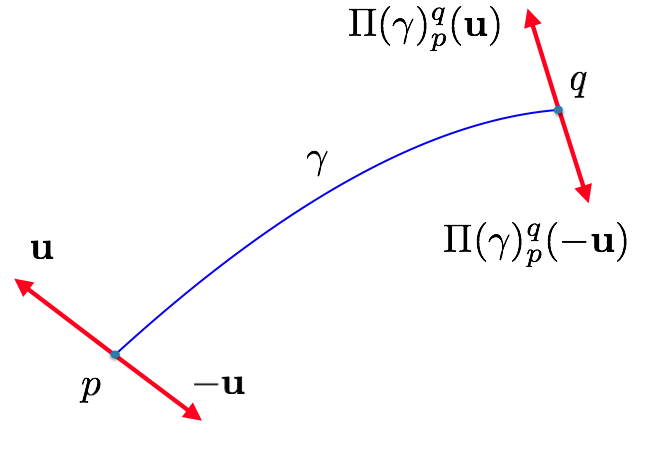
\includegraphics[width=6.5cm]{figures/inversion_1.png}
		\caption{First inversion property.}
		\label{fig:inversion_propr1}
	\end{minipage}
	\ \hspace{9mm} \
	\begin{minipage}[b]{4cm}
		\centering
		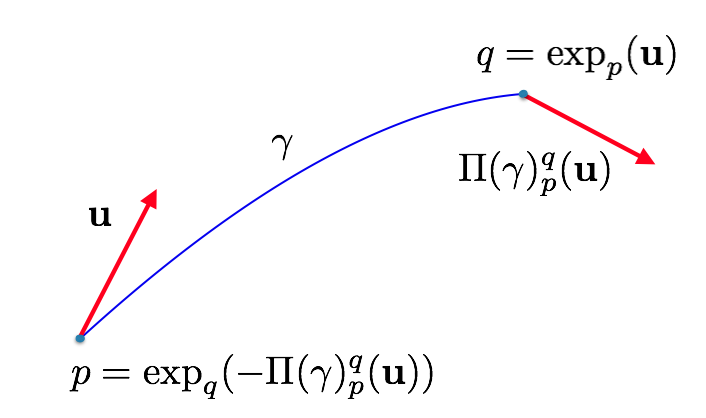
\includegraphics[width=6.5cm]{figures/inversion_2.png}
		\caption{Second inversion property.}
		\label{fig:inversion_propr2}
	\end{minipage}
\end{figure}
\begin{prop}[change of signs of the composition for affine exponential]
	$\mathbb{G}$ Lie group, $\nabla$ connection, $a,b\in\mathbb{G}$, $\mathbf{u}\in T_{a}\mathbb{G}$, $\mathbf{v}\in T_{b}\mathbb{G}$. Let $\beta$ be the tangent curve to $\mathbf{u}$ at $a$ and $c= \exp_{b}(\mathbf{v})$. Given $\mathbf{w} \in T_{c}\mathbb{G}$ such that 
	\begin{align*}
	\exp_{a}(\mathbf{w}) = \exp_{b}(\mathbf{v}) \circ \exp_{a}(\mathbf{u})
	\end{align*}
	Then
	\begin{align*}
	\exp_{a}(-\mathbf{w}) = \exp_{\tilde{b}}(-\Pi(\beta)_{b}^{\tilde{b}}(\mathbf{v})) \circ \exp_{a}(-\mathbf{u})
	\end{align*}
	where $\tilde{b}$ is the affine exponential of $-\mathbf{u}$ or the element $\beta(-1)$.
\end{prop}


\begin{figure}[htbp]
	\centering
	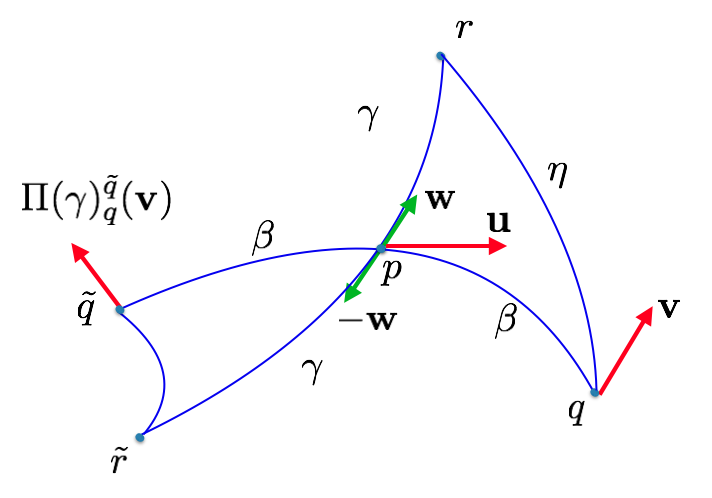
\includegraphics[width=9.5cm]{figures/sign_1.png}
	\caption{Change of sign property.}
	\label{fig:sign_propr}
\end{figure}

\begin{lemma}
	$\mathbb{G}$ Lie group, $\nabla$ connection, $a\in\mathbb{G}$, $\mathbf{u}\in T_{e}\mathbb{G}$. Let $\gamma$ be a curve defined on $\mathbb{G}$ such that $\gamma(0) = e$, $\gamma(1) = a$, $\dot{\gamma}(0) =\mathbf{u}$. Let $\beta$ be the curve over $\mathbf{G}$ defined as $\beta(t) = a\circ \gamma(t)$, then the two following conditions hold:
	\begin{enumerate}
		\item If $\nabla$ is a Cartan connection then $\beta$ is a geodesic.
		\item For $\mathbf{u}_{a} := D(L_{a})_{e}(\mathbf{u}) \in T_{a}\mathbb{G}$, push forward of the left-translation:
		\begin{align}\label{eq:lemma_pt}
		\exp_{a}(t\mathbf{u}_{b}) = b\circ \exp_{e}( t D(L_{a^{-1}})_{a}(\mathbf{u}_{a}) ) = b\circ \exp_{e}(t\mathbf{u})
		\end{align}
	\end{enumerate}
\end{lemma}

\begin{figure}[htbp]
	\centering
	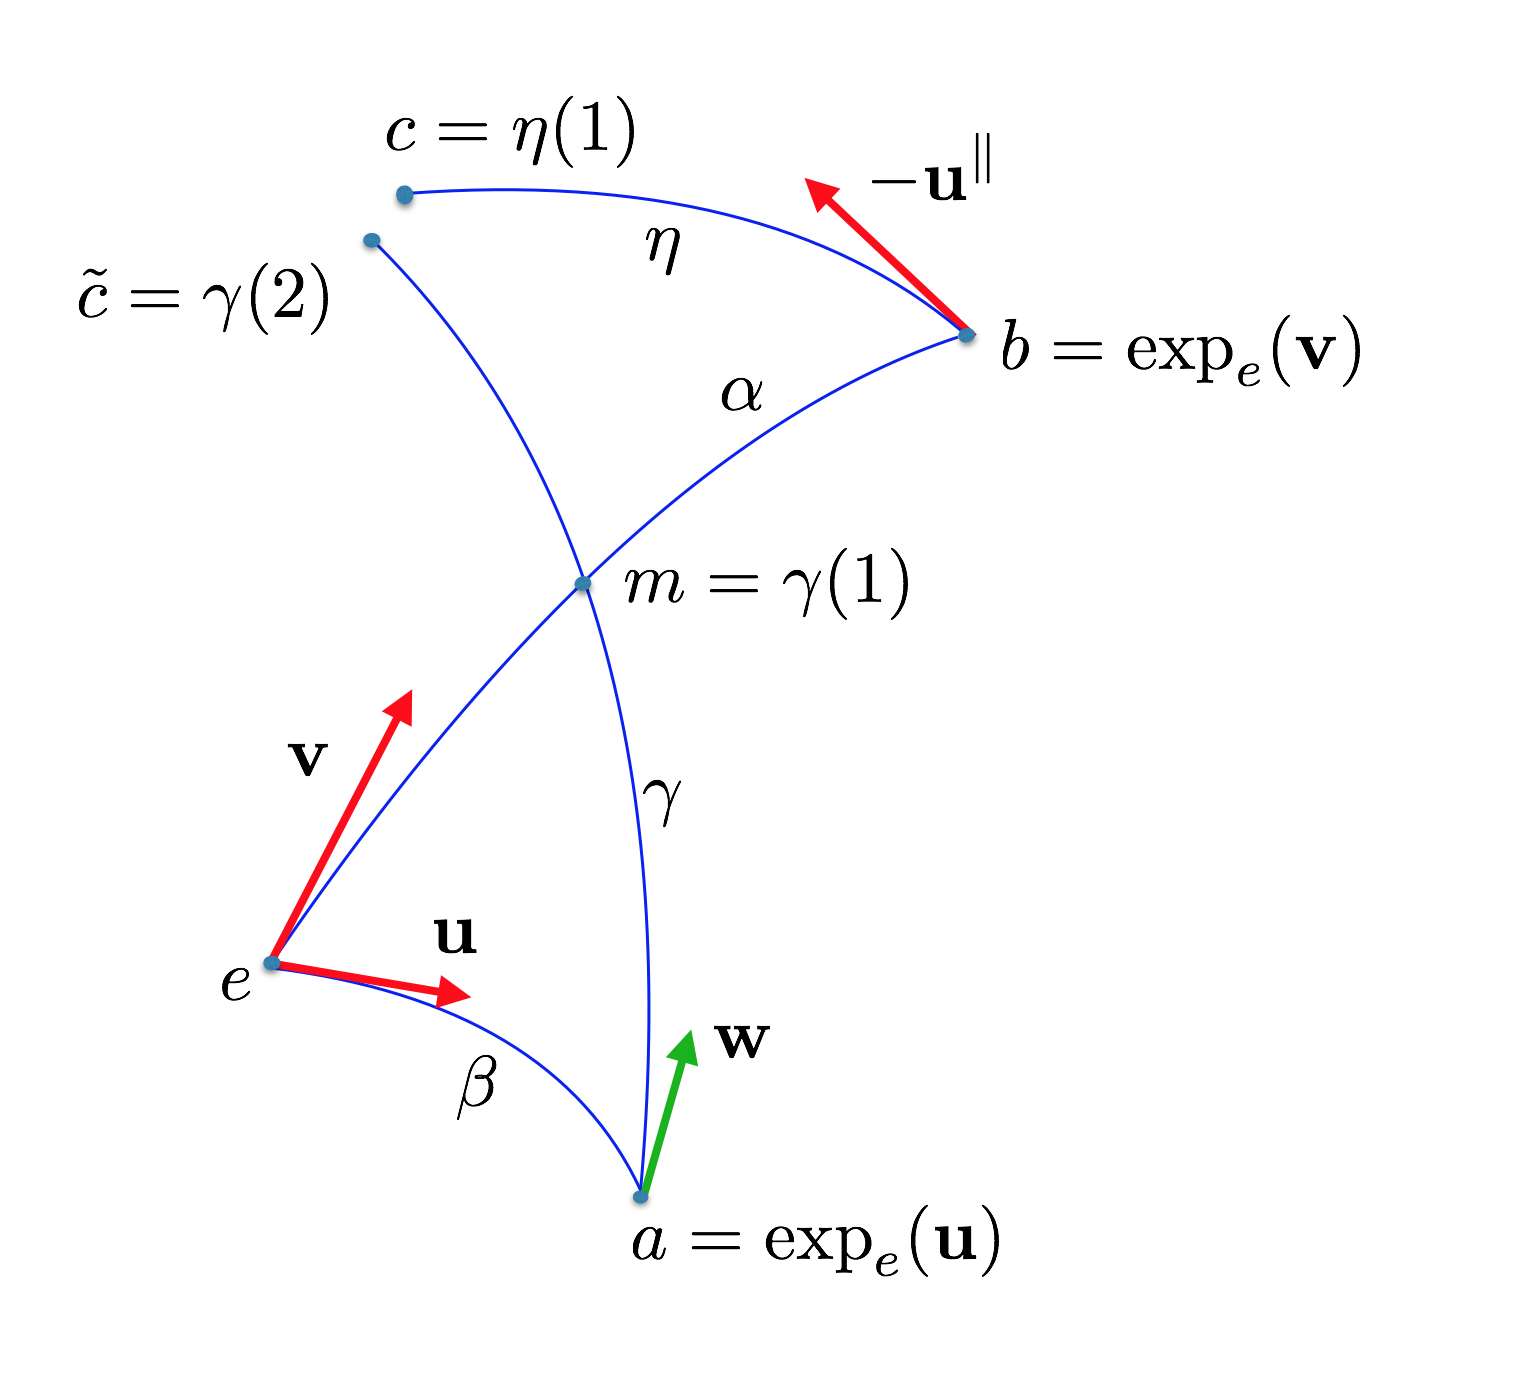
\includegraphics[width=9.5cm]{figures/theorem_pict.png}
	\caption{Pole ladder applied to parallel transport.}
	\label{fig:theorem_pict}
\end{figure}
\noindent
The following theorem is an application of the pole ladder \cite{lorenzi2011schild} for the computation of the exponential that will underpin one of the numerical methods for the computation of the log-composition.
\begin{theorem}\label{th:local_approximation_theorem}
	Let $\mathbb{G}$ be a finite dimensional connected Lie group defined with a Cartan connection $\nabla$. 
	If, for each couple of linearly independent vectors $\mathbf{u}, \mathbf{v} \in T_{e}\mathbb{G}$, we consider the following elements:
	\begin{align*}
	a= \exp_{e}(\mathbf{u}) 
	\quad & \quad  
	b= \exp_{e}(\mathbf{v}) \\
	\mathbf{u}^{\parallel} = & \Pi(\alpha)_{e}^{b}(\mathbf{u})\\
	\gamma : [0,1] \rightarrow \mathbb{G} &\quad \gamma(0) = e \quad \dot{\gamma}(0) = \mathbf{v}
	\end{align*}
	Then, for $\mathbf{u}_{e}^{\parallel} := D(L_{b^{-1}})_{e}( -\Pi(\alpha)_{a}^{b}(\mathbf{u}))$, the approximation
	\begin{align*}
	\exp_{e}(\mathbf{u}_{e}^{\parallel}) 
	\simeq
	\exp_{e}\big(\frac{\mathbf{v}}{2}\big)   
	\circ  \exp_{e}(\mathbf{u}) 
	\circ \exp_{e}\big(-\frac{\mathbf{v}}{2}\big)
	\end{align*}
	holds.
\end{theorem}

%\begin{proof}
%	As a consequence of the construction we have the following considerations:
%	\begin{align*}
%	\gamma(t) &= \exp(t\mathbf{w}) 
%	= 
%	a \circ \exp_{e}(D(L_{ba^{-1}})_{e}(t\mathbf{w})) 
%	= 
%	\exp_{e}(\mathbf{u})  \circ \exp_{e}(D(L_{a^{-1}})_{e}(t\mathbf{w})) 
%	\\
%	m &= \alpha(\frac{1}{2}) 
%	= \exp_{e}\big(\frac{\mathbf{v}}{2}\big) = \gamma(1) = \exp_{a}(\mathbf{w})
%	\\
%	\exp_{e}&(D(L_{a^{-1}})_{e}(\mathbf{w})) = \exp_{e}(-\mathbf{u}) \circ  \exp_{e}\big(\frac{\mathbf{v}}{2}\big) 
%	\end{align*}
%	Let $\eta$ be the integral curve of  $-\Pi(\alpha)_{a}^{b}(\mathbf{u})$ starting at $b$. If $c := \eta(1)$ and $\tilde{c} := \gamma(1)$, then on one side we have:
%	\begin{align*}
%	\tilde{c} = \gamma(1) &= \exp_a(2\mathbf{w}) = a \circ\exp_{e}(D(L_{a^{-1}})_{e}(2\mathbf{w})) \\
%	&= \exp_{e}(\mathbf{u})\circ\exp_{e}(D(L_{a^{-1}})_{e}(\mathbf{2w})) \\
%	&= \exp_{e}(\mathbf{u})\circ\exp_{e}(2D(L_{a^{-1}})_{e}(\mathbf{w})) \\
%	&= \exp_{e}(\mathbf{u})\circ \big(\exp_{e}(D(L_{a^{-1}})_{e}(\mathbf{w})) \big)^2\\
%	&=  \exp_{e}(\mathbf{u})\circ \big(  \exp_{e}(-\mathbf{u}) \circ  \exp_{e}(\frac{\mathbf{v}}{2}) \big)^2\\
%	&=   \exp_{e}\big(\frac{\mathbf{v}}{2}\big)   
%	\circ  \exp_{e}(-\mathbf{u}) 
%	\circ \exp_{e}\big(\frac{\mathbf{v}}{2}\big) 
%	\end{align*}
%	On the other side:
%	\begin{align*}
%	c = \eta(1) &= \exp_{b}(-\mathbf{u}^{\parallel}) = b \circ\exp_{e}(D(L_{b^{-1}})_{e}(-\mathbf{u}^{\parallel})) \\
%	&= \exp_{e}(\mathbf{v}) \circ\exp_{e}(D(L_{b^{-1}})_{e}(-\mathbf{u}^{\parallel})) \\
%	&= \exp_{e}(\mathbf{v}) \circ\exp_{e}(-\mathbf{u}_{e}^{\parallel}) 
%	\end{align*}
%	where $D(L_{b^{-1}})_{e}(\mathbf{u}^{\parallel})$ has been written $\mathbf{u}_{e}^{\parallel}$ for brevity.
%	If we consider $c\simeq \tilde{c}$ it follows that:
%	\begin{align*}
%	\exp_{e}\big(\frac{\mathbf{v}}{2}\big)   
%	\circ  \exp_{e}(-\mathbf{u}) 
%	\circ \exp_{e}\big(\frac{\mathbf{v}}{2}\big)
%	\simeq
%	\exp_{e}(\mathbf{v}) \circ\exp_{e}(-\mathbf{u}_{e}^{\parallel}) 
%	\end{align*}
%	which implies
%	\begin{align*}
%	\exp_{e}(-\mathbf{u}_{e}^{\parallel}) 
%	&\simeq
%	\exp_{e}(-\mathbf{v}) 
%	\circ \exp_{e}\big(\frac{\mathbf{v}}{2}\big)   
%	\circ  \exp_{e}(-\mathbf{u}) 
%	\circ \exp_{e}\big(\frac{\mathbf{v}}{2}\big)
%	\\
%	\exp_{e}(-\mathbf{u}_{e}^{\parallel}) 
%	&\simeq
%	\exp_{e}\big(-\frac{\mathbf{v}}{2}\big)   
%	\circ  \exp_{e}(-\mathbf{u}) 
%	\circ \exp_{e}\big(\frac{\mathbf{v}}{2}\big)
%	\end{align*}
%	As a consequence of property of the signs inversion it follows that
%	\begin{align*}
%	\exp_{e}(\mathbf{u}_{e}^{\parallel}) 
%	\simeq
%	\exp_{e}\big(\frac{\mathbf{v}}{2}\big)   
%	\circ  \exp_{e}(\mathbf{u}) 
%	\circ \exp_{e}\big(-\frac{\mathbf{v}}{2}\big)
%	\end{align*}
%\end{proof} 

\begin{corollary}
	xxx attempt to measure the error in the formula... to be done in a more effective way!
	If, with previous notations, the condition (1) is an approximation
	\begin{align*}
	\exp_{C}(\frac{\mathbf{k}}{2}) = \exp(\mathbf{\xi})\circ \exp_{M}(\frac{\mathbf{k}}{2}) 
	\end{align*}
	for some $ \mathbf{\xi}$ in  $\mathfrak{g}$ such that $\parallel\mathbf{\xi} \parallel < \delta$
	then the approximation has error
	\begin{align*}
	O(\parallel \delta\mathbf{u}^{\parallel} \parallel^{2} )  
	+ O(\parallel \mathbf{u} + \delta\mathbf{u}\parallel^{3})
	+ \text{xxx something that must be investigated depending on } \delta
	\end{align*}
\end{corollary}



% % % % % % % % % % % % % % % % % % % % % % % % % % % % % % % % % % % % % %
In considering the equation \ref{eq:lemma_pt} we used implicitly the formula for the change of base for affine exponential and logarithm. It is in fact possible, using the derivative of the left-translation $L_{p}$, to bring back the $\exp$ and the $\log$ functions based at the point $p$ of the manifold to the $\exp$ and the $\log$ evaluated at the identity using the following formulas:
\begin{align}\label{eq:DL_DR}
\log _{p}(q)  &= DL_{p}(e) \log _{e}(q)  \\
\exp _{p}(\mathbf{u})  &= p\circ \exp_{e} (DL_{p}(e)^{-1} \mathbf{u})
\end{align}
\noindent
The interested reader can refer to the extended version on github \cite{xxx}, where proofs and examples are provided and relations between \ref{eq:DL_DR} and parallel transport are investigated.




% % % % % % % % % % % % % % % % % % % % % % % % % % % % % % % % % % % % % %
% % SECTION
% % % % % % % % % % % % % % % % % % % % % % % % % % % % % % % % % % % % % %
\section{Four Strategies for the Computation of Log-composition}

In this section we provide explicit formulas for the computation of the log composition, using the tools introduced in the previous sections.

% % % % % % % % % % % % % % % % % % % % % % % % % % % % % % % % % % % % % %
% % SUBSECTION
% % % % % % % % % % % % % % % % % % % % % % % % % % % % % % % % % % % % % % 
\subsection{Truncated BCH formula}\label{se:bch_formula}

To compute the Lie Log composition, literature provides the BCH formula, defined as the solution of the equation $exp(\mathbf{w}) = \exp(\mathbf{u}) \circ \exp(\mathbf{v})$, for $\bf{u}$ and $\bf{v}$ in the Lie algebra $\mathfrak{g}$:
\begin{align*}
	BCH(\mathbf{u},\mathbf{v}) 
	= 
	\mathbf{u} + \mathbf{v} + \frac{1}{2}[\mathbf{u},\mathbf{v}] + \frac{1}{12}([\mathbf{u},[\mathbf{u},\mathbf{v}]]
	+ [\mathbf{v},[\mathbf{v},\mathbf{u}]]) - \frac{1}{24}[\mathbf{v},[\mathbf{u},[\mathbf{u},\mathbf{v}]]] +... 
\end{align*}

\noindent
xxx derivation of the bch formula, constraints on the Lie algebra elements involved in its computation.


% % % % % % % % % % % % % % % % % % % % % % % % % % % % % % % % % % % % % %
% % SUBSECTION
% % % % % % % % % % % % % % % % % % % % % % % % % % % % % % % % % % % % % % 
\subsection{Taylor Expansion}\label{se:taylor_expansion}

Once \emph{adjoint action} of $\mathbf{u}$ on the Lia algebra is defined, nested Lie bracket can be reformulated as multiple composition of this operator:
\begin{align*}
ad_{\mathbf{u}} : \mathfrak{g}  & \longrightarrow \mathfrak{g}  
\\
\mathbf{v} &\longmapsto ad_{\mathbf{u}}   =  [\mathbf{u}, \mathbf{v}]
\end{align*}
So
\begin{align*}
[  \underbrace{   \mathbf{u},[\mathbf{u},... [\mathbf{u}}_{\text{n-times}},\mathbf{v}]...]] =  ad_{\mathbf{u}}^{n}(\mathbf{v})
\end{align*}
In the appendix of xxx Klarsfeld xxx adjoint action are used to provide an expansion of the BCH formula. This can be rewritten as
\begin{align*}
\mathbf{u}\oplus \mathbf{v}  = \mathbf{u} + \frac{ ad_{\mathbf{u}} \exp(ad_{\mathbf{u}}) }{ \exp(ad_{\mathbf{u}}) - 1 }  \mathbf{v} + O({\mathbf{v}}^2)
\end{align*}

\noindent
xxx intermediate passages to be written from zachos, blane!

The functional applied to $\mathbf{v}$ can be rewritten as
\begin{align*}
\frac{ ad_{\mathbf{u}} \exp(ad_{\mathbf{u}}) }{ \exp(ad_{\mathbf{u}}) - 1 }  = \sum_{n=0}^{\infty} \frac{B_{n}}{n!} ad_{\mathbf{u}}^{n} 
\end{align*}
Where $\lbrace B_{n} \rbrace $ is the sequence of the second-kind Bernoulli number\footnote{If first-kind Bernoulli number is used then each term of the summation must be multiplied for $(-1)^{n}$, as did for example in ....Klarsfeld.}.

% % % % % % % % % % % % % % % % % % % % % % % % % % % % % % % % % % % % % %
% % SUBSECTION
% % % % % % % % % % % % % % % % % % % % % % % % % % % % % % % % % % % % % % 
\subsection{Parallel Transport}




\subsection{Numerical Computations of the Log-composition for SE(n)}


\subsubsection{Taylor Approximation to compute the Log-composition}

We can apply the Taylor expansion formula for the computation of the affine log-composition to matrices in $SE(2)$.
From previous subsection we have:
\begin{align*}
\mathbf{u}\star \mathbf{v}  = \mathbf{u} + \frac{ ad_{\mathbf{u}} \exp(ad_{\mathbf{u}}) }{ \exp(ad_{\mathbf{u}}) - 1 }  \mathbf{v} + O({\mathbf{v}}^2)
\qquad
\frac{ ad_{\mathbf{u}} \exp(ad_{\mathbf{u}}) }{ \exp(ad_{\mathbf{u}}) - 1 }  = \sum_{n=0}^{\infty} \frac{B_{n}}{n!} ad_{\mathbf{u}}^{n} 
\end{align*}
Where $\lbrace B_{n} \rbrace $ is the sequence of the second-kind Bernoulli number\footnote{If first-kind Bernoulli number is used then each term of the summation must be multiplied for $(-1)^{n}$, as did for example in ....Klarsfeld.}.



\subsubsection{Parallel Transport to compute the Log-composition}




\subsubsection{Log and Exp Approximations for Small Rotations}
Computations of logarithm and exponential obtained so far are a consequence of these formula:
\begin{align*}
\exp(\mathbf{r}) = \sum_{k=0}^{\infty} \frac{\mathbf{v}^{k}}{k!}
\qquad 
\log(\mathbf{r}) = \sum_{k=1}^{\infty}(-1)^{k+1} \frac{(\mathbf{v}-I)^{k} }{k!}
\end{align*}
Remarkably, infinite series of elements of a group (whose sum is not even defined within the group structure) is an element into an associated algebra, while another infinite series of matrices of the algebra appears to be the natural way to going backward. A second door to passing from one structure to the other, when $\mathbf{r}$ is little appears to be the following approximation:
\begin{align*}
\exp(\mathbf{r}) \simeq I + \mathbf{r} 
\qquad 
\log(d\mathbf{r}) \simeq d\mathbf{r} - I
\end{align*}
In fact for little $\theta$, $\sin(\theta) \simeq \theta$, $\cos(\theta) \simeq 0 $ and $ L(\theta)^{-1} \simeq I$. \\
xxx this may deserve an investigation about the errors in the approximations error!



